\section{Modeling Extra-functional Properties}\label{sec_extrafunc}
In this section, we discuss the timing, application reliability, and power consumption models used throughout the paper.

\subsection{Power Consumption Model}
Power consumption refers to the energy per time unit usage of electronic components in an integrated circuit, e.g., processor, memory, I/O devices, etc. Depending on the nature of the integrated circuit and intended use, there exist various techniques of estimating power and energy consumption. For instance, measuring power consumption of flip-flop and combinatorial gates in CMOS-based integrated circuits, also known as \textit{low-level models }\cite{Najm1994ACircuits}\cite{Najm1995PowerCircuits}, are frequently used in the design of power-efficient electronic circuits designs,  and dynamic profiling of computer components, e.g., CPU, memory, I/O devices, etc., are used to construct \textit{high-level models} which primarily used in energy management software, e.g., in dynamic Voltage and Frequency Scaling (DVFS) \cite{Contreras2005PowerEvents}.

However, the previously mentioned methods are limited for our use for two main reasons: i) lack of complete and accurate information of electrical specification of integrated circuits makes the use of low-level power estimation methods difficult; ii) dynamic profiling requires runtime mechanisms, such as performance counter monitor. Instead, in this work, we employ a different approach which makes use of processor load (or \textit{Processor Utilization}) to estimate the average power consumption of a computational node. Specifically, we use the linear polynomial model proposed by Fan et al. \cite{Fan2007PowerComputer}, which is shown in (\ref{eqn_powerconsumption}). 
\begin{equation}
\label{eqn_powerconsumption}
p(u)=P_{idle} + (P_{busy}-P_{idle})*u
\end{equation}

The power consumption model contains two important parameters: the $p_{idle}$ and $p_{busy}$, respectively refer to the power consumption of a node measured at minimum and maximum processor loads. Such measurements can be conducted, for instance by running power or performance benchmark suits, e.g., MiBench \cite{Guthaus2001MiBench:Suite}, AutoBench \cite{EMBC2018AutoBenchProcessors}, etc.
\begin{figure*}[h!]
    \centering
    \begin{subfigure}[b]{0.25\textwidth}
    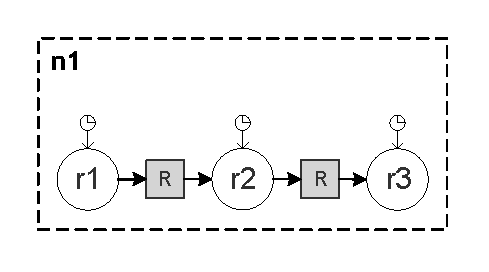
\includegraphics[width=\textwidth]{datachain_singlenode}
    \caption{Deployment on a single node.}
    \label{fig_datachainsingle}
    \end{subfigure}
    ~ %\quad, \qquad, \hfill 
    \begin{subfigure}[b]{0.35\textwidth}
    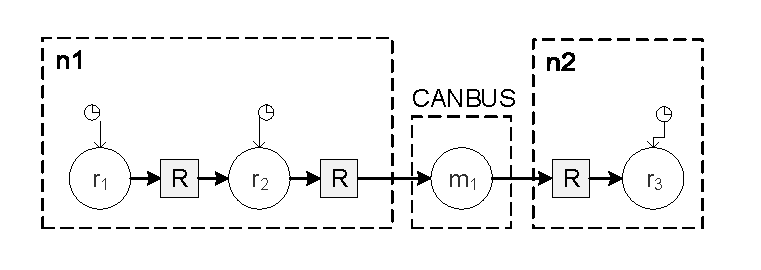
\includegraphics[width=\textwidth]{datachain_multinode}
    \caption{Deployment on multiple nodes,}
    \label{fig_datachainmulti}
    \end{subfigure}
   \hfill
    \begin{subfigure}[b]{0.375\textwidth}
    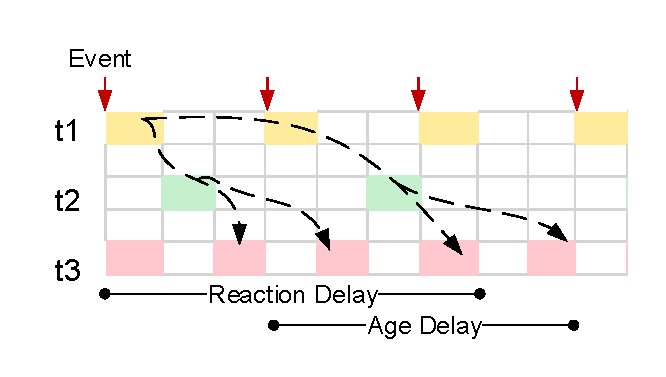
\includegraphics[width=\textwidth]{timedpath}
    \caption{Timed Paths of Age and Reaction Delays}
    \label{fig_timedpath}
    \end{subfigure}
    \caption{Cause-effect chain with three activation patterns.}
    \label{fig:datachain}
\end{figure*}

\subsection{Software Application Reliability}
\textit{Application reliability} $R_a$ refers to the probability that a software application functions correctly by the time $t$, or within the time interval $[0, t]$ \cite{Goel1985SoftwareApplicability}. We assume that  applications are free from design errors and, therefore, an application failure can be caused only by failures from computational nodes in which the application is deployed. The failure-rate of a node over time is represented by $\lambda(t)$ and its reliability, by $\lambda e^{-\lambda t}$ for constant failure-rate and exponential density function. 

In a system without replication, the failure of any arbitrary node would make the whole application faulty. Reliability calculation in these conditions is straightforward, using a series-parallel model: $R_a = \prod_{m\in M}r_m$.

Introduction of replication for fault tolerance creates interdependencies between nodes executing replicas of the same software component, and makes the calculation more complicated. An application will \textit{function correctly} if each software component is executed at least by one non-faulty node, and will be \textit{faulty} otherwise (i.e., if there are one or more software components that are allocated only to faulty nodes and thus these components cannot be executed correctly).

To calculate the reliability in such cases, we use \textit{State Enumeration}, which is one of the reliability-preserving methods that are used to compute reliability of a system with dependent components (or subsystems) \cite{Lucet1999ExactReliability}. The State Enumeration method allows the exploration of all possible states of a system in the probability space $P\!S$. Our goal is to differentiate between the states in which the application functions, denoted $\mbox{\it Functions(s)}$, and the states in which the application fails, denoted $\mbox{\it Fails(s)}$. Such that the application reliability $R_a$ is calculated as follows:
\begin{equation}
\label{eqn_appreliability}
R_a=\sum_{s\in PS|Functions(s)}p_s=1-\sum_{s\in PS|Fails(s)}p_s
\end{equation}

To obtain $p_s$, the probability that the application is in state $s\in PS$, we define the boolean variable $z_m \in \{0,1\}$ to indicate whether a node $m \in M$ is either faulty, $z_m = 0$, or not, $z_m = 1$. The probability is then calculated with this equation:
\begin{align}
\label{eqn_stateprobability}
p_s=\prod_{m\in M}((z_m*r_m) + (1-z_m)*(1-r_m))
\end{align}

\subsection{The Timing Model}
The software application can be considered as a set of cause-effect chains, which are directed paths in the application graph. Each cause-effect chains is annotated with an end-to-end timing requirement that specifies the maximum time between the stimuli and response of a chain, for instance, activation of a cruise control system using the rotary wheel located in the dashboard, slowing down a car by pressing the brake pedal of a car, etc. A cause-effect chain can be hosted on a single node or multiple nodes as illustrated in Figure \ref{fig_datachainsingle} and Figure \ref{fig_datachainmulti}, respectively. Moreover, it can be activated by a single or multiple activation patterns, which are a set of clock events that trigger the start of Runnables execution. 

In multi-rate systems, the data-propagation delay calculations in cause-effect chains are not trivial due to the \textit{oversampling} and \textit{undersampling} effects, caused by the different time domains, e.g., tasks communicating with different periodic time events. Consequently, there can be different timed paths through which the data can propagate from the input to the output of the chain, resulting in different delay semantics~\cite{mubeen2013support}. In this work, we focus on the \textit{Age} and \textit{Reaction} delays, which are the most widely used delay semantics in the automotive embedded systems. The two delays in a cause-effect chain that is distributed over two nodes  are demonstrated in Figure~\ref{fig_timedpath}. The tasks t1 and t2 execute on one node, whereas task t3 executes on the second node. Note that t2 communicates with t3 via a network message which is not shown in the figure for simplicity. The red inverted arrows in Figure~\ref{fig_timedpath} represent the arrival of events at the input of the chain, whereas the dashed-curve arrows represent the timed paths through which the data propagates from the input to the output of the chain. The Age delay is the time elapsed between the stimuli and its corresponding latest non-overwritten response, i.e., between the $2^{nd}$ instance of t1 and the $5^{th}$ instance of t3. This delay is frequently used in the control systems applications where freshness of data is paramount. For example, the torque applied to turn the wheels must correspond to the position of the steering wheel and must be time bound. Whereas, the Reaction delay is the earliest time the system takes to respond to a stimuli that ``just missed" the read access at the input of the chain. Assume that an event occurs just after the start of execution of the $1^{st}$ instance of t1. The data corresponding to this event is not read by the current instance of t1. In fact, the data will be read by the $2^{nd}$ instance of t1. The earliest effect of this event at the output of the chain will appear at the $4^{th}$ instance of t3, which represents the reaction delay. This delay is useful in body-electronics domain where first reaction to events is important, e.g., in the button-to-reaction applications. We refer the reader to \cite{mubeen2013support} for the formal semantics of the two delays used in this paper.
